\section{Metodología de trabajo}

\begin{slide}
  \begin{block}{\textbf{Prototipado evolutivo}}
    \begin{center}
      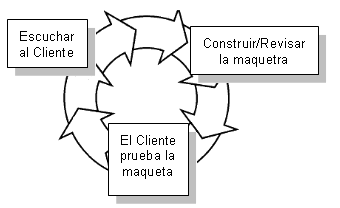
\includegraphics[height=0.5\textheight]{img/prototipo.png}
    \end{center}
  \end{block}
\end{slide}

\begin{slide}
  \begin{block}{\textbf{Iteraciones}}
    \begin{itemize}
      \item Mostrar mapa
      \item Mostrar posición en el mapa
      \item Orientar el mapa
      \item Crear y mostrar ruta
      \item Navegar por una ruta
      \item Selector de destino
      \item Avisos por pantalla
      \item Avisos sonoros
      \item Avisos vibratorios
    \end{itemize}
  \end{block}
\end{slide}

\begin{slide}
  \begin{figure}[!h]
    \begin{center}
      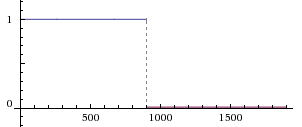
\includegraphics[height=0.25\textheight]{img/graficaGiro.png}
      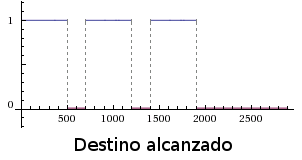
\includegraphics[height=0.25\textheight]{img/graficaDestino.png}
    \end{center}
  \end{figure}
  \begin{figure}[!h]
    \begin{center}
      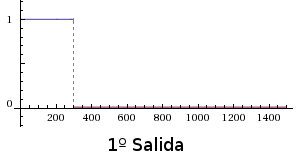
\includegraphics[height=0.21\textheight]{img/graficaRotonda1.png}
      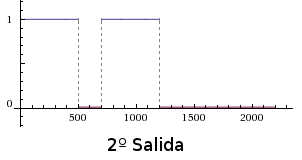
\includegraphics[height=0.21\textheight]{img/graficaRotonda2.png}
      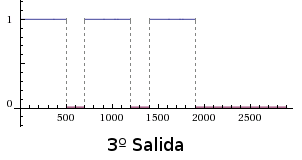
\includegraphics[height=0.21\textheight]{img/graficaRotonda3.png}
    \end{center}
  \end{figure}
\end{slide}

% Local Variables:
%  TeX-master: "main.tex"
%  coding: utf-8
%  mode: latex
%  mode: flyspell
%  ispell-local-dictionary: "castellano8"
% End:
